
\section{Estimates for number of Monte-Carlo samples needed}
\label{sec:experiments}

Lemma \ref{lemma:mcmc-numinf} in Section \ref{sse:poly} shows that an 
$(\epsilon, \delta)$-approximation to the expected total number of infections 
in a set $S$ up to time $t$ can be estimated in polynomial time by a simple
Monte-Carlo sampling approach. Here, we examine the empirical complexity
of Monte-Carlo sampling of other problems in Table \ref{tab:prob_def}.
As an example, let $p^*$ be the exact probability for an instance of the \tTotInfs{} problem.
We use the approach of Dagum et al. \cite{dagum:focs95}, which gives an
$(\epsilon, \delta)$-approximation to $p^*$ using 
$N_{\epsilon, \delta} = O(N_{opt})$ samples, where
$N_{\epsilon, \delta}$ is the number of samples used by \cite{dagum:focs95}, and
$N_{opt}$ is the optimum number of Monte-Carlo samples that can give such an approximation
to $p^*$.  Figure \ref{fig:dagum-mcmc} shows $N_{\epsilon, \delta}$ as a function
of $t$ for a social contact network for Montgomery county, VA, 
constructed using the approach of \cite{eubank:nature04, barrett:wsc09},
for a probability $p$, which ensures that the expected number of infections
is close to 15\% of the number of nodes.
We note that $N_{\epsilon, \delta}$ are quite high.

\begin{figure}
\centering
%%\includegraphics[width=0.4\textwidth]{{dagum-0.0002}.pdf}
%%\includegraphics[width=0.4\textwidth]{{dagum-0.0004}.pdf}
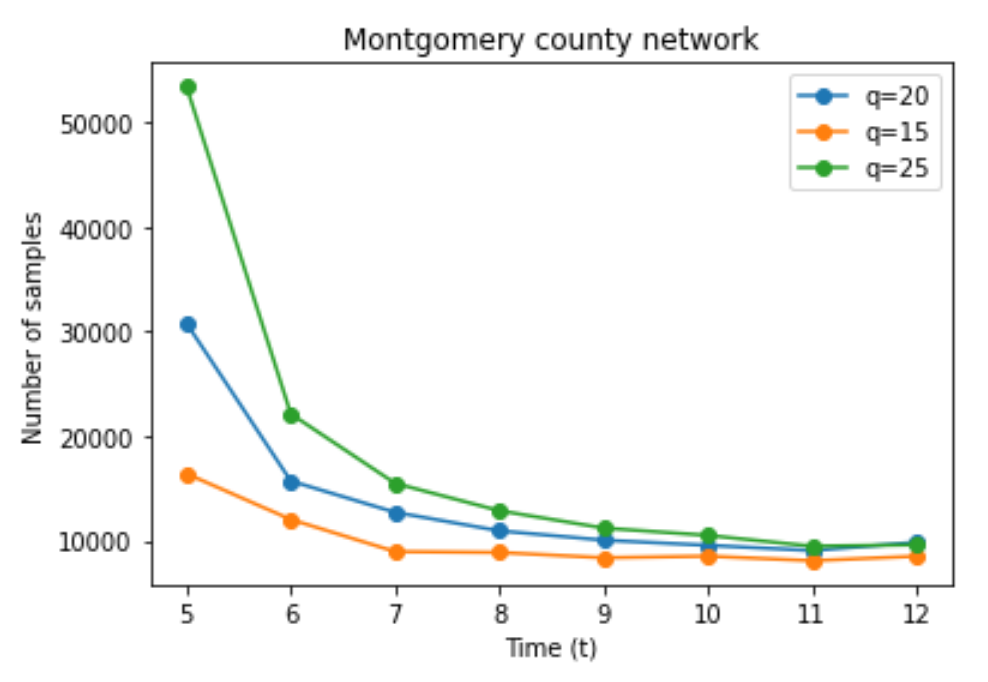
\includegraphics[width=0.4\textwidth]{montgomery.png}
\caption{Number of Monte-Carlo samples using the approach of Dagum et al. \cite{dagum:focs95}
on a social contact network for Montgomery county, VA, constructed using the approach of
\cite{eubank:nature04, barrett:wsc09},
for a transmission probability, such that the expected number of infections 
is around 15\% of the total number of nodes.
}
\label{fig:dagum-mcmc}
\end{figure}

